\documentclass[12pt, a4paper, oneside]{ctexart}
\usepackage{amsmath, amsthm, amssymb, bm, caption,  color, enumerate, float, framed, graphicx, hyperref,listings, mathrsfs, subfigure}
\usepackage[usenames,dvipsnames]{xcolor}

\definecolor{mygreen}{rgb}{0,0.6,0}
\definecolor{mygray}{rgb}{0.5,0.5,0.5}
\definecolor{mymauve}{rgb}{0.58,0,0.82}
\lstset{ %
backgroundcolor=\color{white},   % choose the background color
basicstyle=\footnotesize\ttfamily,        % size of fonts used for the code
columns=fullflexible,
breaklines=true,                 % automatic line breaking only at whitespace
captionpos=b,                    % sets the caption-position to bottom
tabsize=4,
commentstyle=\color{mygreen},    % comment style
escapeinside={\%*}{*)},          % if you want to add LaTeX within your code
keywordstyle=\color{blue},       % keyword style
stringstyle=\color{mymauve}\ttfamily,     % string literal style
frame=single,
rulesepcolor=\color{red!20!green!20!blue!20},
% identifierstyle=\color{red},
language=c++,
}





\title{\textbf{实验一\ 排序算法\ 实验报告}}
\author{PB18061443 江昊霖}
\date{\today}
\linespread{1.5}

\newenvironment{problem}{\begin{shaded}\stepcounter{problemnum}\par\noindent\textbf{题目\arabic{problemnum}. }}{\end{shaded}\par}
\newenvironment{solution}{\par\noindent\textbf{解答. }}{\par}

\begin{document}

\maketitle

\section{实验内容}

\begin{enumerate}
    \item 排序n个元素, 元素为随机生成的0到$2^{15} - 1$之间的整数, n的取值为:
          $2^3, 2^6, 2^9, 2^{12}, 2^{15}, 2^{18}$。
    \item 实现以下算法: 堆排序, 快速排序, 归并排序, 计数排序。
\end{enumerate}

\section{实验设备和环境}

\begin{figure}[htbp]
    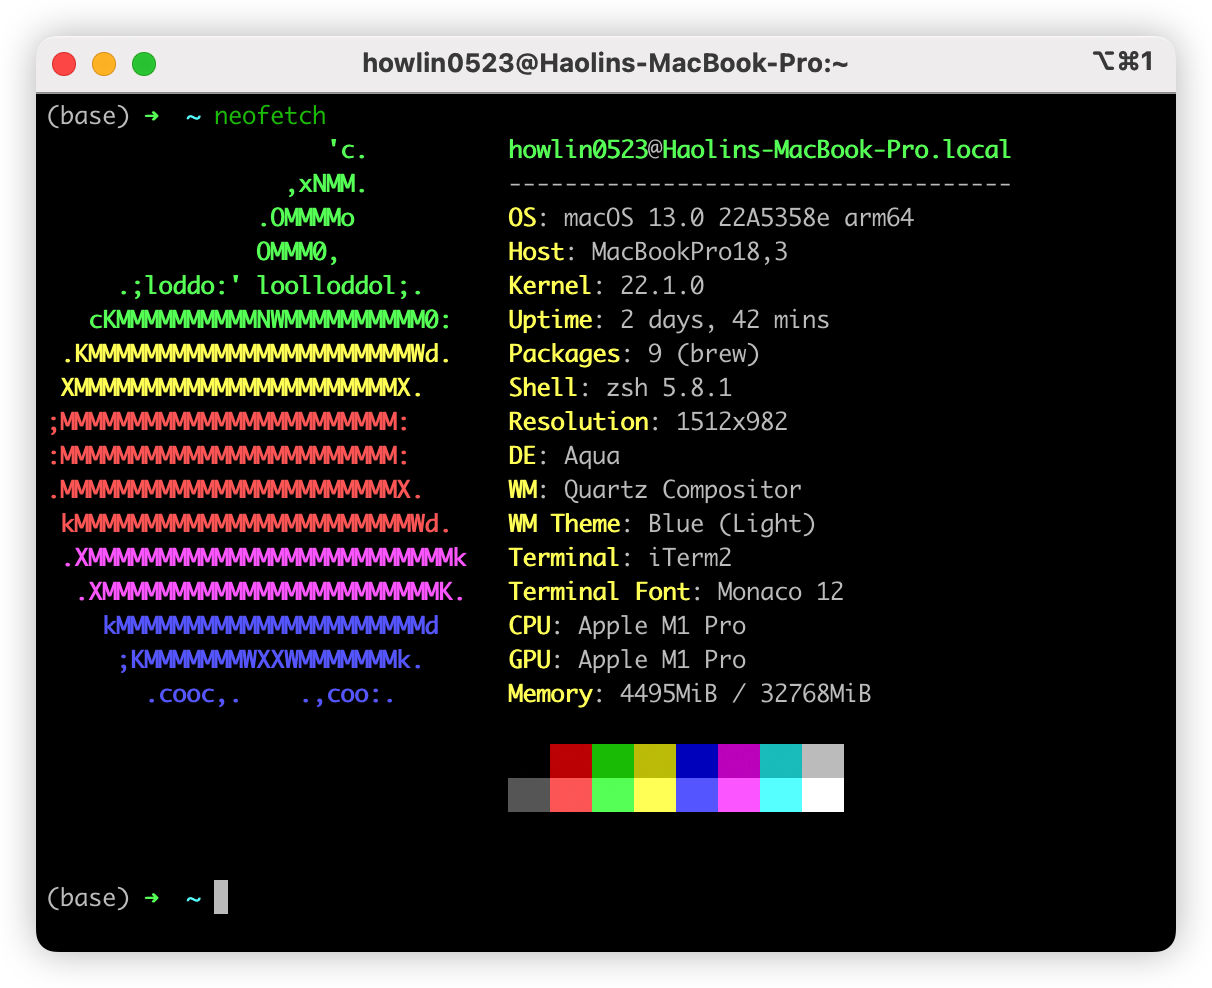
\includegraphics[width = 0.5\textwidth]{./image/info.png}
    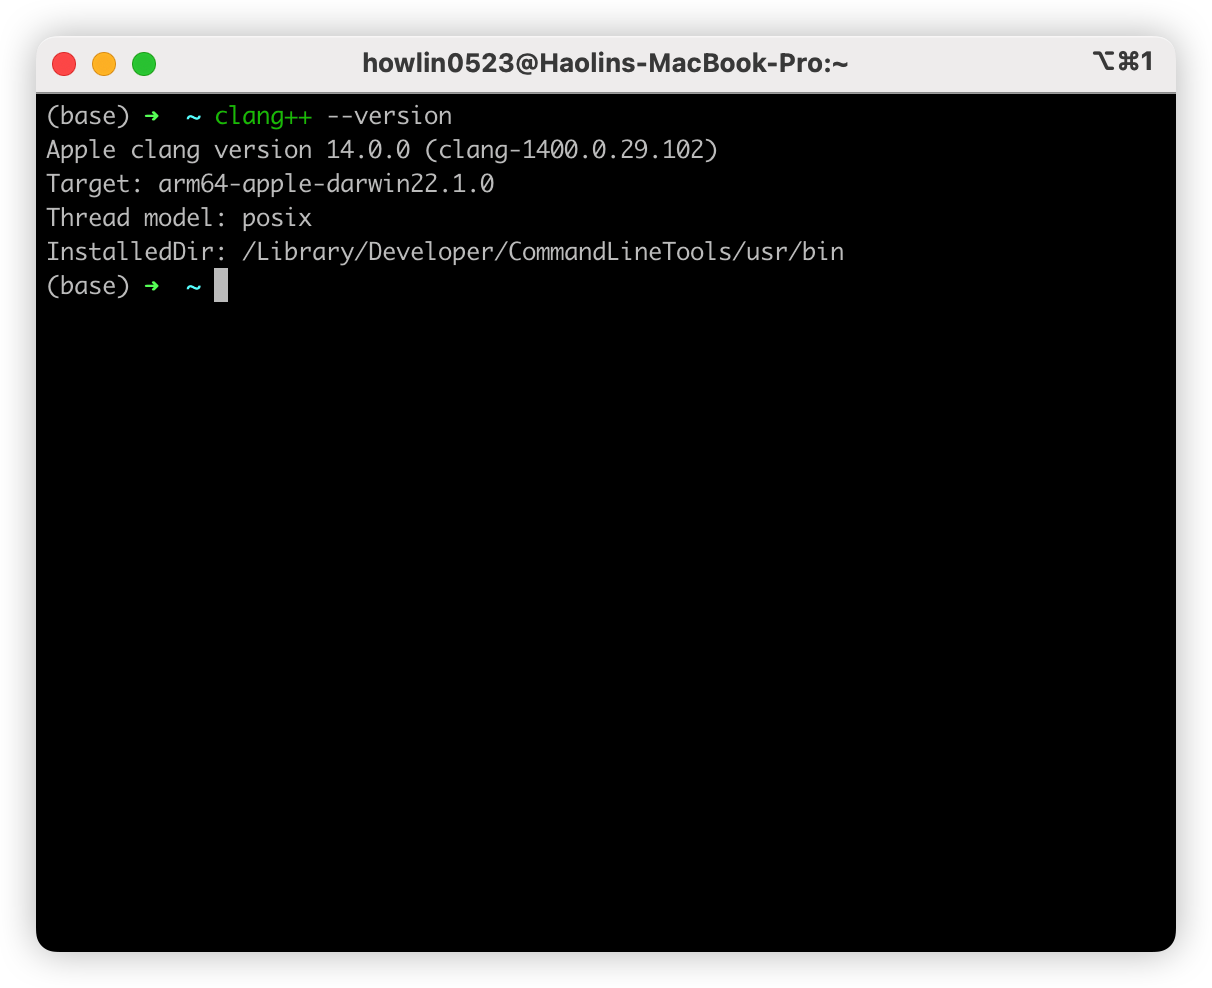
\includegraphics[width = 0.5\textwidth]{./image/clang.png}
\end{figure}

\section{实验方法和步骤}

\subsection{堆排序}

\begin{lstlisting}
void heapify(vector<int> &arr, int N, int i)
{
	int largest = i;

	int left = 2 * i + 1;
	int right = 2 * i + 2;

	if (left < N && arr[left] > arr[largest])
		largest = left;

	if (right < N && arr[right] > arr[largest])
		largest = right;

	if (largest != i)
	{
		swap(&arr[i], &arr[largest]);
		heapify(arr, N, largest);
	}
}
	
void heapSort(vector<int> &arr, int N)
{
	for (int i = N / 2 - 1; i >= 0; i--)
		heapify(arr, N, i);

	for (int i = N - 1; i >= 0; i--)
	{
		swap(&arr[0], &arr[i]);
		heapify(arr, i, 0);
	}
}
\end{lstlisting}



\subsection{快速排序}


\begin{lstlisting}
int partition(vector<int> &arr, int low, int high)
{
    int pivot = arr[high];
    int i = (low - 1);

    for (int j = low; j <= high - 1; j++)
    {

        if (arr[j] < pivot)
        {
            i++;
            swap(&arr[i], &arr[j]);
        }
    }
    swap(&arr[i + 1], &arr[high]);
    return (i + 1);
}

void quickSort(vector<int> &arr, int low, int high)
{
    if (low < high)
    {

        int pi = partition(arr, low, high);

        quickSort(arr, low, pi - 1);
        quickSort(arr, pi + 1, high);
    }
}
\end{lstlisting}
\subsection{归并排序}

\begin{lstlisting}
void merge(vector<int> &arr, int front, int mid, int end)
{
    vector<int> LeftSubarr(arr.begin() + front, arr.begin() + mid + 1);
    vector<int> RightSubarr(arr.begin() + mid + 1, arr.begin() + end + 1);
    int idxLeft = 0, idxRight = 0;
    LeftSubarr.insert(LeftSubarr.end(), numeric_limits<int>::max());
    RightSubarr.insert(RightSubarr.end(), numeric_limits<int>::max());
    for (int i = front; i <= end; i++)
    {
        if (LeftSubarr[idxLeft] < RightSubarr[idxRight])
        {
            arr[i] = LeftSubarr[idxLeft];
            idxLeft++;
        }
        else
        {
            arr[i] = RightSubarr[idxRight];
            idxRight++;
        }
    }
}

void mergeSort(vector<int> &arr, int front, int end)
{
    if (front >= end)
        return;
    int mid = (front + end) / 2;
    mergeSort(arr, front, mid);
    mergeSort(arr, mid + 1, end);
    merge(arr, front, mid, end);
}
\end{lstlisting}

\subsection{计数排序}

\begin{lstlisting}
void countingSort(vector<int> &arr)
{
    int max = *max_element(arr.begin(), arr.end());
    int min = *min_element(arr.begin(), arr.end());
    int range = max - min + 1;

    vector<int> count(range), output(arr.size());
    for (int i = 0; i < arr.size(); i++)
        count[arr[i] - min]++;

    for (int i = 1; i < count.size(); i++)
        count[i] += count[i - 1];

    for (int i = arr.size() - 1; i >= 0; i--)
    {
        output[count[arr[i] - min] - 1] = arr[i];
        count[arr[i] - min]--;
    }

    for (int i = 0; i < arr.size(); i++)
        arr[i] = output[i];
}
\end{lstlisting}


\section{实验结果与分析}
\begin{figure*}[htbp]
    \centering
    \begin{subfigure}[堆排序]{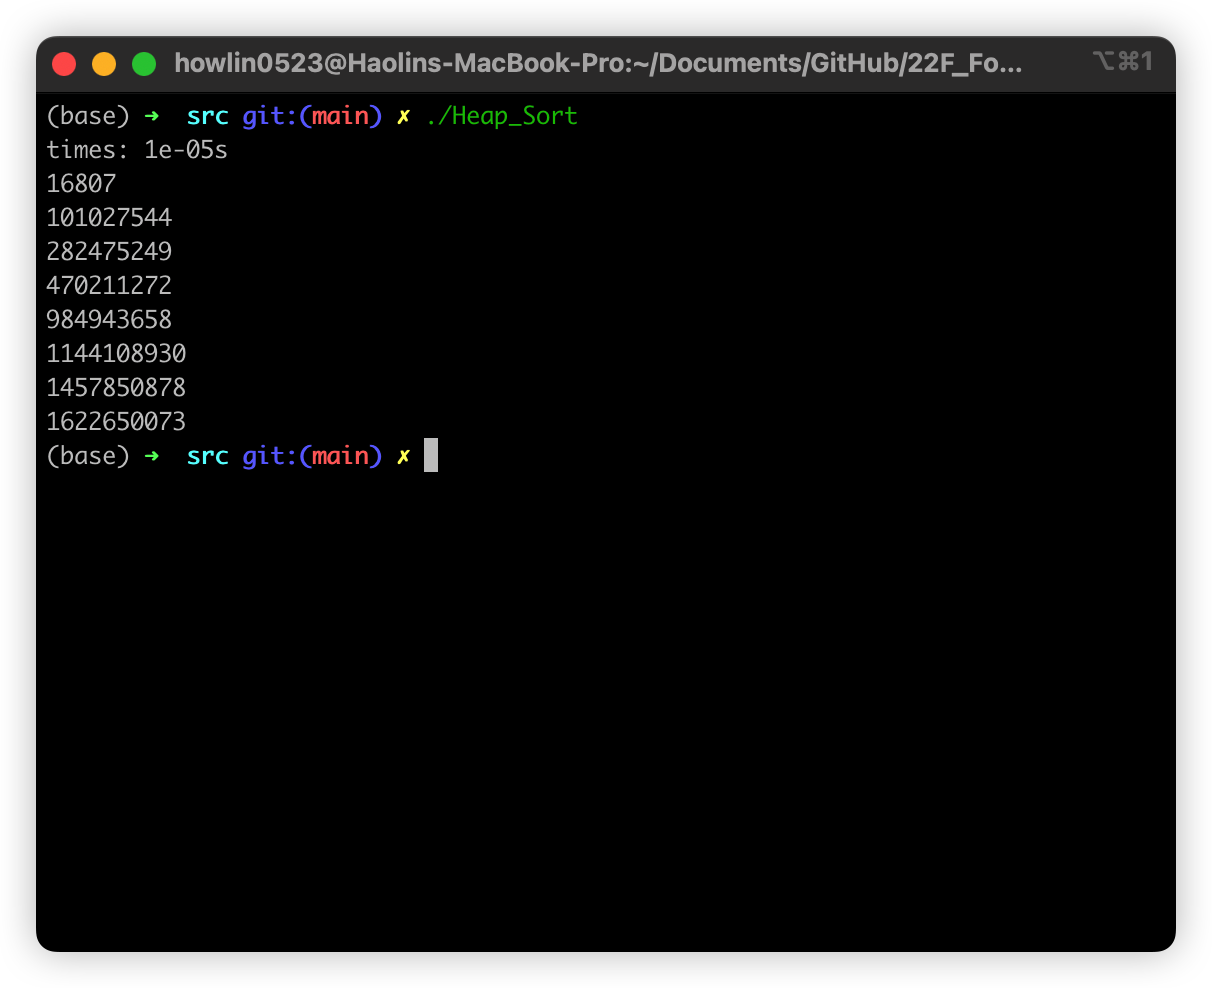
\includegraphics[width = 0.45\textwidth]{image/heapSort.png}}
    \end{subfigure}
    \begin{subfigure}[快速排序]{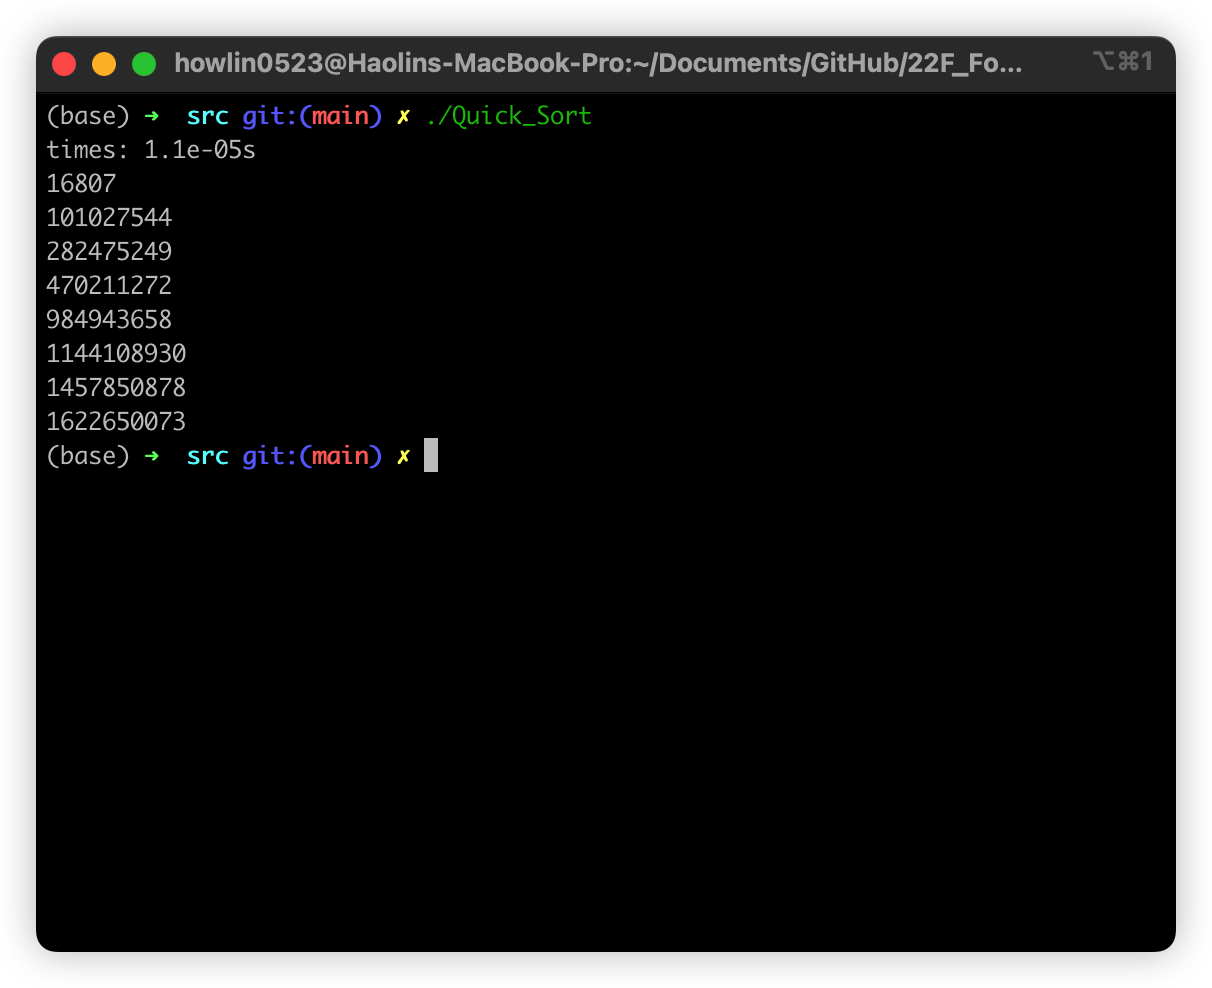
\includegraphics[width = 0.45\textwidth]{image/quickSort.png}}
    \end{subfigure}\\
    \begin{subfigure}[归并排序]{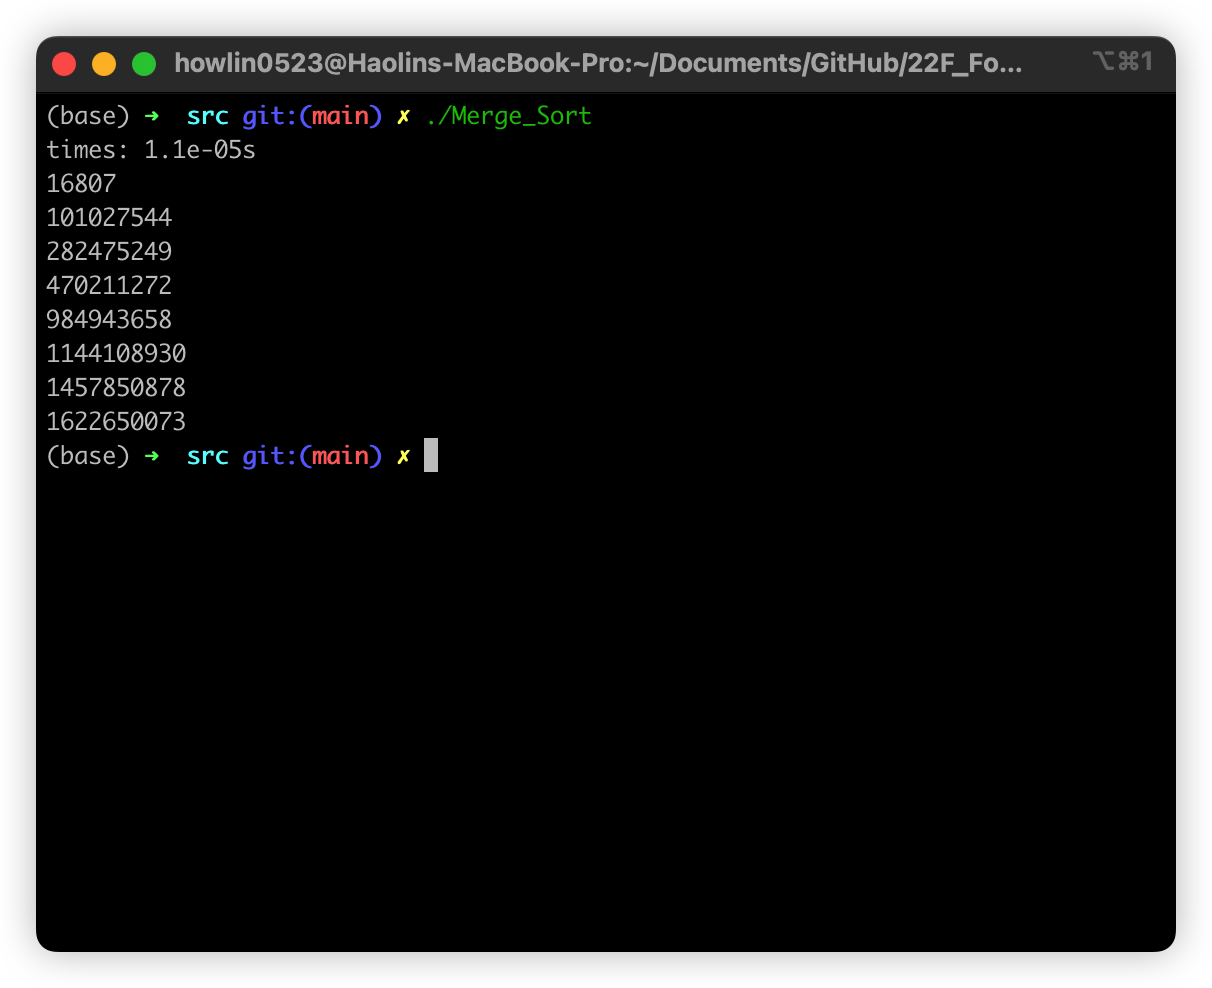
\includegraphics[width = 0.45\textwidth]{image/mergeSort.png}}
    \end{subfigure}
    \begin{subfigure}[计数排序]{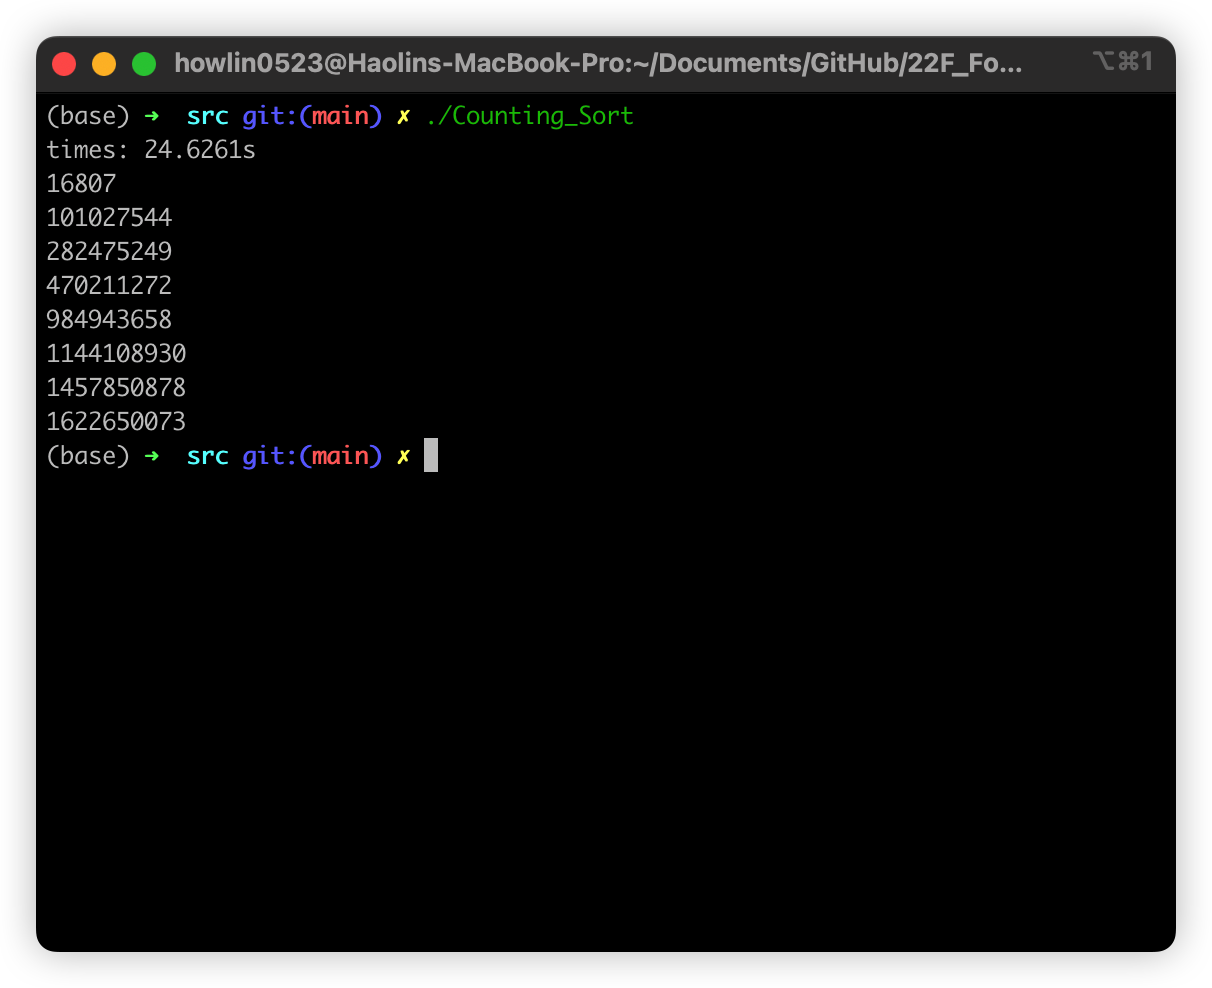
\includegraphics[width = 0.45\textwidth]{image/countingSort.png}}
    \end{subfigure}
    \caption{$n=2^3$时排序结果}
\end{figure*}

\begin{figure*}[htbp]
    \centering
    \begin{subfigure}[堆排序]{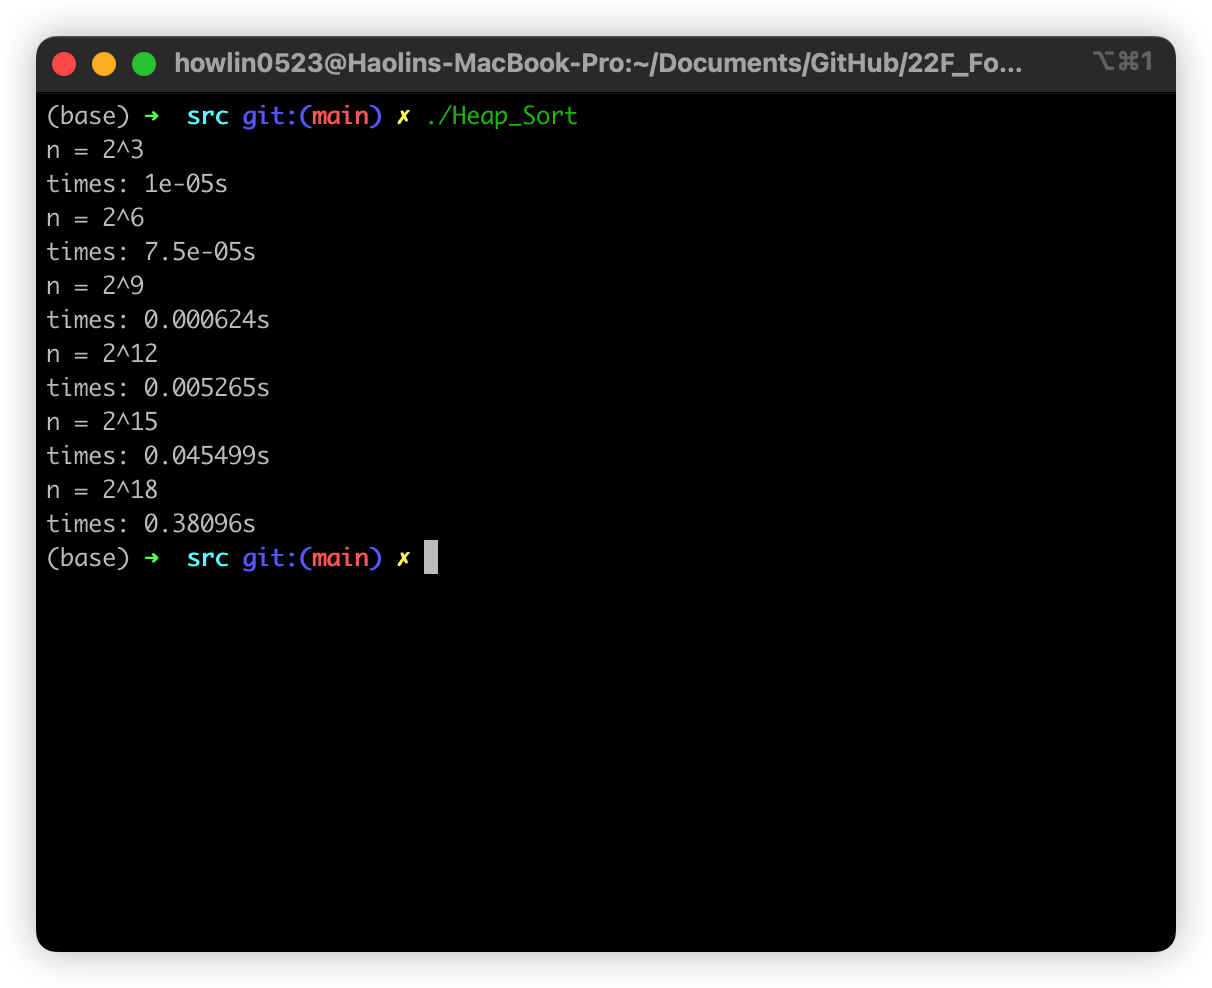
\includegraphics[width = 0.45\textwidth]{image/heapSort_all.png}}
    \end{subfigure}
    \begin{subfigure}[快速排序]{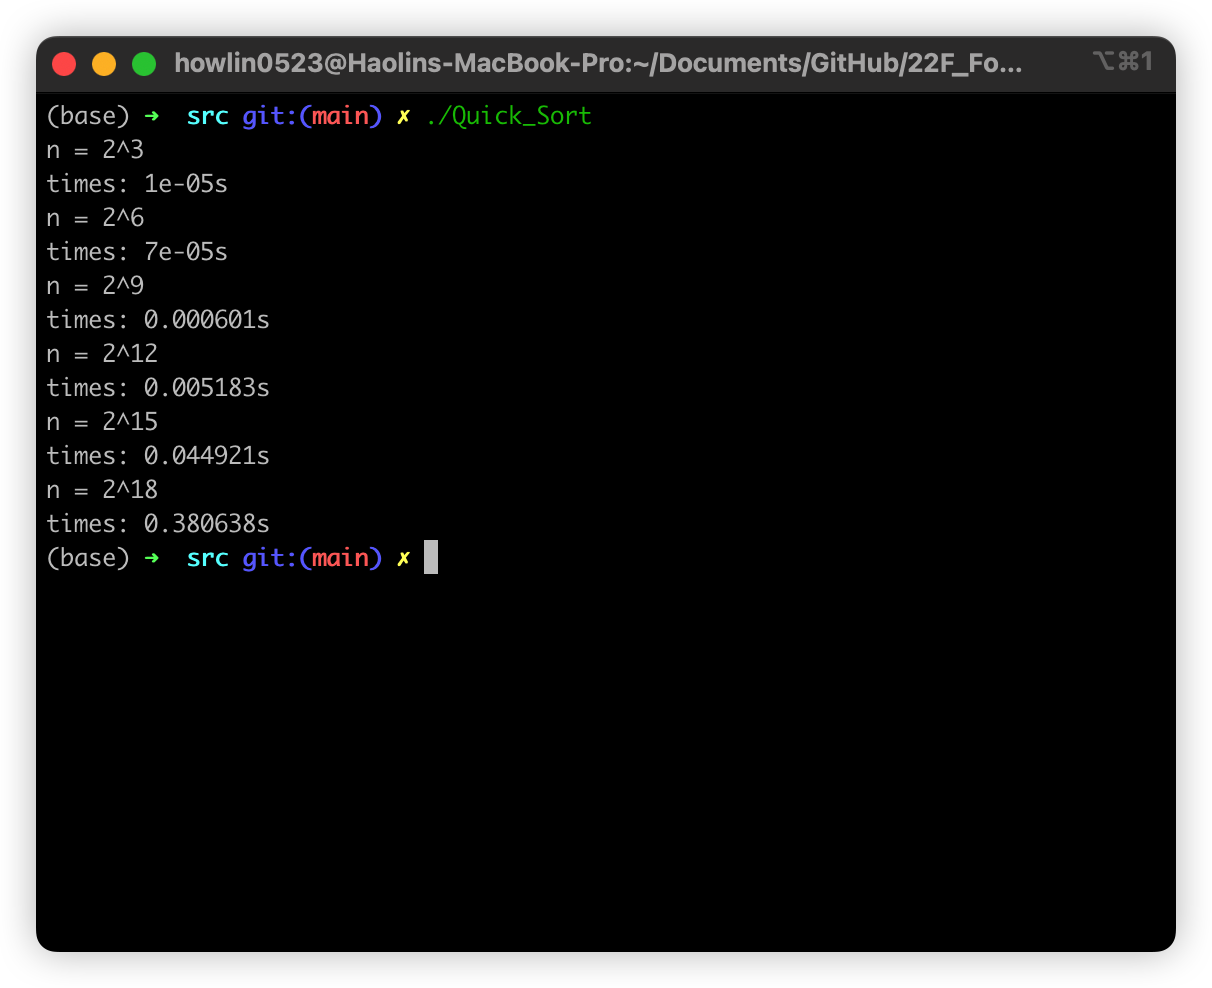
\includegraphics[width = 0.45\textwidth]{image/quickSort_all.png}}
    \end{subfigure}\\
    \begin{subfigure}[归并排序]{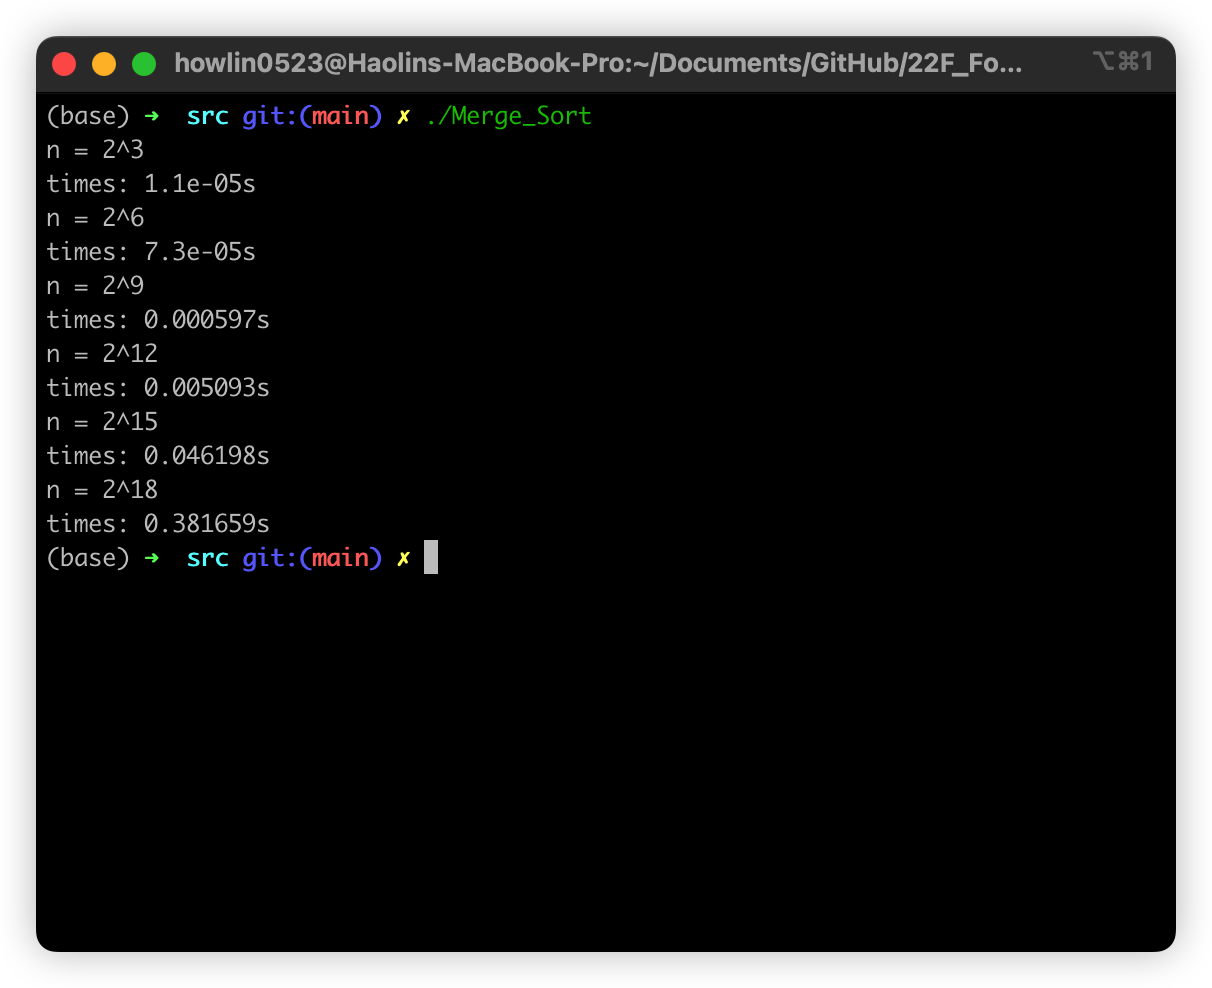
\includegraphics[width = 0.45\textwidth]{image/mergeSort_all.png}}
    \end{subfigure}
    \begin{subfigure}[计数排序]{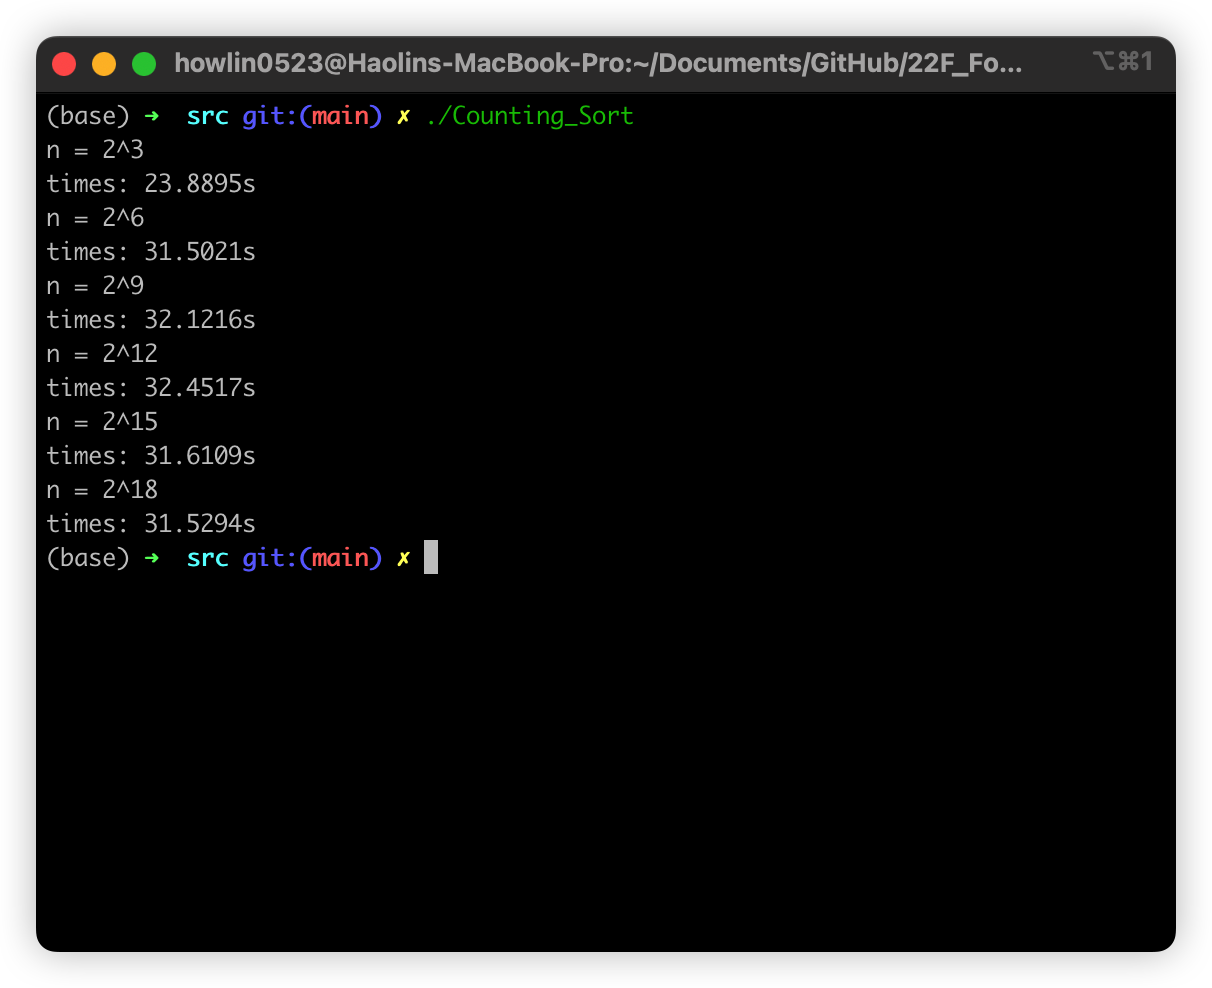
\includegraphics[width = 0.45\textwidth]{image/countingSort_all.png}}
    \end{subfigure}
    \caption{六个输入规模运行时间}
\end{figure*}

\begin{figure*}[htbp]
    \centering
    \begin{subfigure}[堆排序]{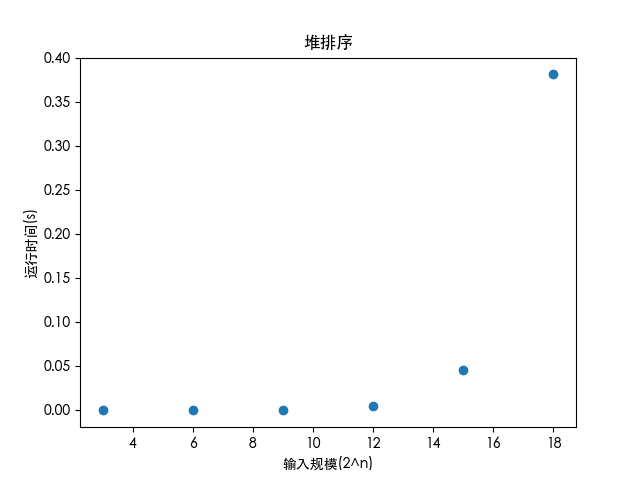
\includegraphics[width = 0.45\textwidth]{image/heapSort_result.png}}
    \end{subfigure}
    \begin{subfigure}[快速排序]{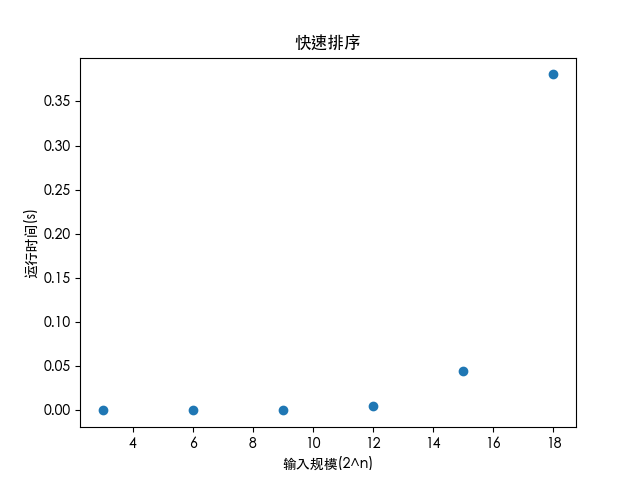
\includegraphics[width = 0.45\textwidth]{image/quickSort_result.png}}
    \end{subfigure}\\
    \begin{subfigure}[归并排序]{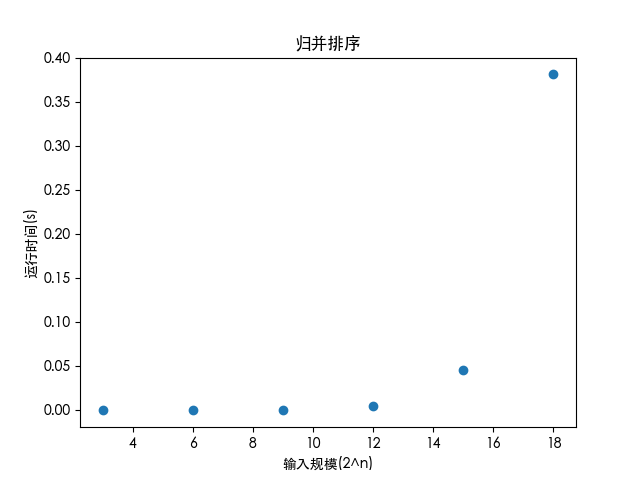
\includegraphics[width = 0.45\textwidth]{image/mergeSort_result.png}}
    \end{subfigure}
    \begin{subfigure}[计数排序]{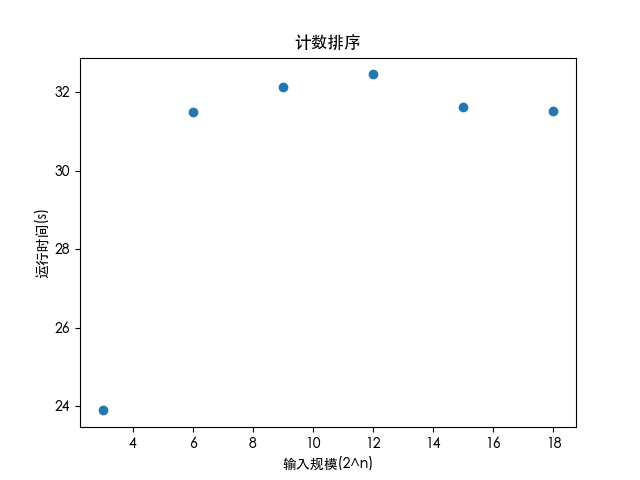
\includegraphics[width = 0.45\textwidth]{image/countingSort_result.png}}
    \end{subfigure}
    \caption{六个输入规模运行时间}
\end{figure*}
\newpage
\subsection*{结果分析}

堆排序、 快速排序、 归并排序的运行时间符合理论时间复杂度$O(n\log n)$, 而计数排序符合$O(n+k)$, 计数排序花的时间相对久是因为需要遍历数组得到$\max$和$\min$


堆排序、 快速排序、 归并排序三个排序算法在6个输入规模下所花的时间差不多, 计数排序由于输入的随机数大小$k\in(0,2^{15}-1)$, 时间复杂度比前三个都要高出不少 




\end{document}